\chapter{Diagrammi}

\section{Strategy Pattern}
Nella programmazione ad oggetti, lo strategy pattern è uno dei pattern fondamentali, definiti originariamente dalla gang of four.

Lo strategy pattern è uno dei pattern comportamentali. L'obiettivo di questa architettura è isolare un algoritmo all'interno di un oggetto. Il pattern strategy è utile in quelle situazioni dove sia necessario modificare dinamicamente gli algoritmi utilizzati da un'applicazione. Si pensi ad esempio alle possibili visite in una struttura ad albero (visita anticipata, simmetrica, posticipata): mediante il pattern strategy è possibile selezionare a tempo di esecuzione una tra le visite ed eseguirla sull'albero per ottenere il risultato voluto. Il design pattern Iterator si basa proprio su questo.

Questo pattern prevede che gli algoritmi siano intercambiabili tra loro (in base ad una qualche condizione) in modo trasparente al client che ne fa uso. In altre parole: la famiglia di algoritmi che implementa una funzionalità (ad esempio di visita o di ordinamento) esporta sempre la medesima interfaccia, in questo modo il client dell'algoritmo non deve fare nessuna assunzione su quale sia la strategia istanziata in un particolare istante.

Nell'applicazione realizzata abbiamo utilizzato questo design pattern per fornire il supporto all'estensione del sistema per l'aggiunta di nuovi algoritmi per l'estrazione delle caratteristiche.

\begin{figure}[ht]
	\centering
	%width=.5\textwidth
	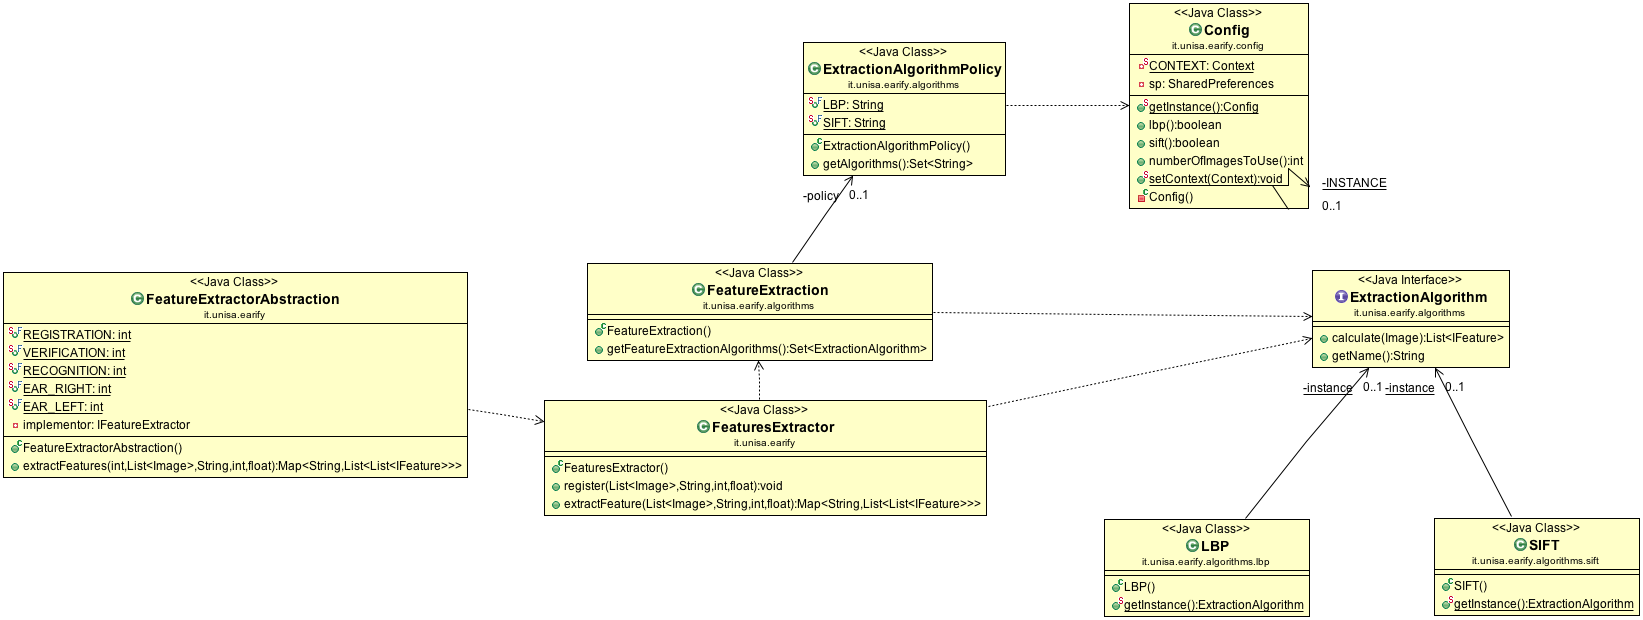
\includegraphics[width=1.5\textwidth, angle=90]{img/strategy.png}
	\caption{Strategy}\label{fig:strategy}
\end{figure}

\section{Bridge Pattern}
Il bridge pattern è un design pattern (modello di progettazione) della programmazione ad oggetti e permette di separare l'interfaccia di una classe (che cosa si può fare con la classe) dalla sua implementazione (come si fa). In tal modo si può usare l'ereditarietà per fare evolvere l'interfaccia o l'implementazione in modo separato.

Abbiamo utilizzato questo design pattern per supportare l'aggiunta di diverse implementazioni del medesimo algoritmo di estrazione. Un esempio di utilizzo di questo pattern può essere individuato nell'implementazione di due versioni dell'algoritmo LBP: una scritta in linguaggio nativo C e l'altra in linguaggio Java.

\begin{figure}[ht]
	\centering
	%width=.5\textwidth
	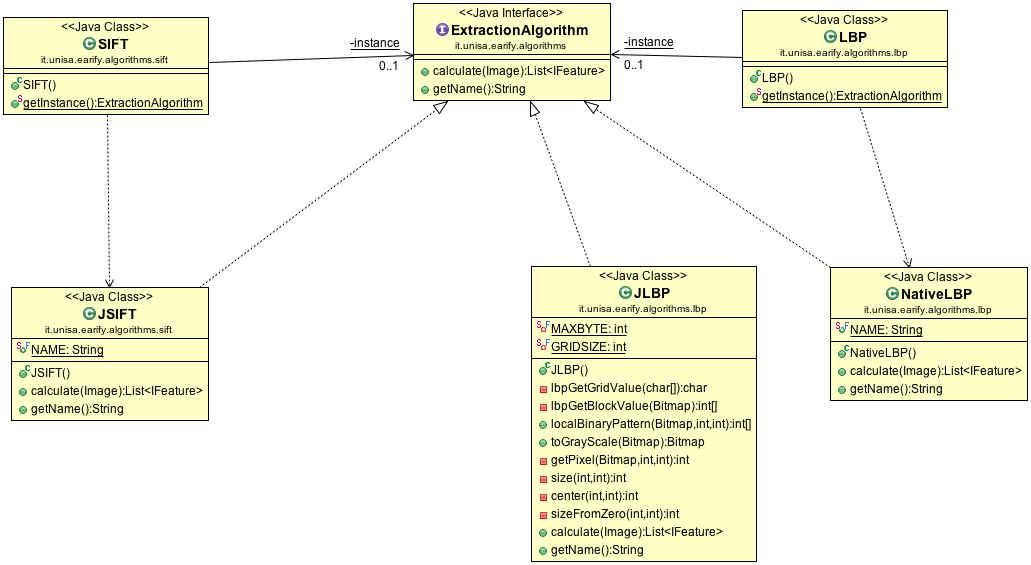
\includegraphics[width=1.5\textwidth, angle=90]{img/bridge.png}
	\caption{Bridge}\label{fig:bridge}
\end{figure}

\section{Observer Pattern}
L'Observer pattern è un design pattern utilizzato per tenere sotto controllo lo stato di diversi oggetti.

È un pattern intuitivamente utilizzato come base architetturale di molti sistemi di gestione di eventi. Molti paradigmi di programmazione legati agli eventi, utilizzati anche quando ancora non era diffusa la programmazione ad oggetti, sono riconducibili a questo pattern. È possibile individuarlo in maniera rudimentale nella programmazione di sistema Windows, o in altri framework di sviluppo che richiedono la gestione di eventi provenienti da diversi oggetti, come ad esempio la funzione "OnMsgProc" per la gestione delle code di messaggi windows.

Sostanzialmente il pattern si basa su uno o più oggetti, chiamati osservatori o listener, che vengono registrati per gestire un evento che potrebbe essere generato dall'oggetto "osservato".

Oltre all'observer esiste il concrete Observer che si differenzia dal primo perché implementa direttamente le azioni da compiere in risposta ad un messaggio; riepilogando il primo è una classe astratta, il secondo no.

Uno degli aspetti fondamentali è che tutto il funzionamento dell'observer si basa su meccanismi di callback, implementabili in diversi modi, o tramite funzioni virtuali o tramite puntatori a funzioni passati quali argomenti nel momento della registrazione dell'observer, e spesso a questa funzione vengono passati dei parametri in fase di generazione dell'evento.

Abbiamo utilizza questo design pattern per fornire un callback alla attività principale dell'applicazione Android al momento in cui il Thread asincrono che effettua l'estrazione tramite gli algoritmi scelti termina la sua esecuzione correttamente o termina a seguito di un'eccezione generata.

\begin{figure}[ht]
	\centering
	%width=.5\textwidth
	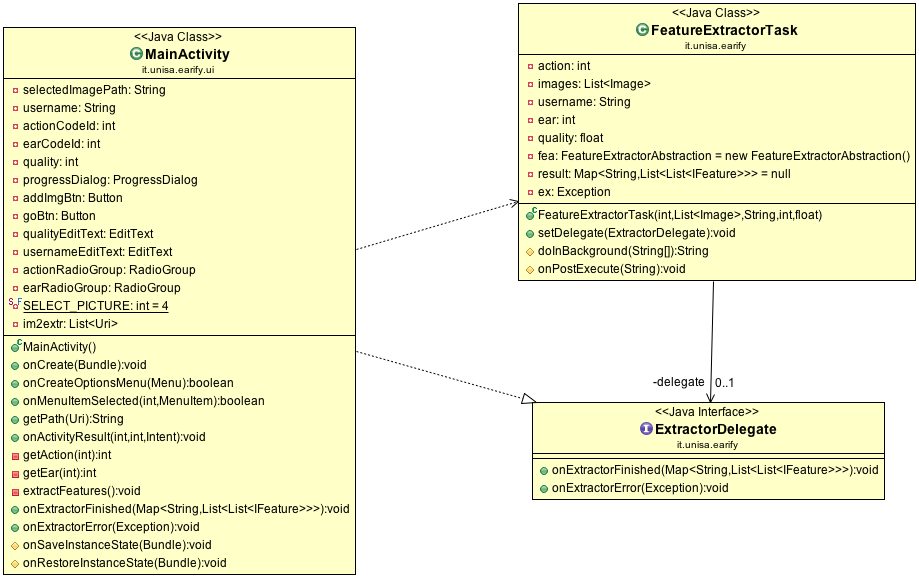
\includegraphics[width=1.5\textwidth, angle=90]{img/delegation.png}
	\caption{Observer}\label{fig:delegation}
\end{figure}

\section{Pacchetti}
L'applicazione si dipana nei pacchetti rappresentati in figura \ref{fig:pkg}.

\begin{figure}[ht]
	\centering
	%width=.5\textwidth
	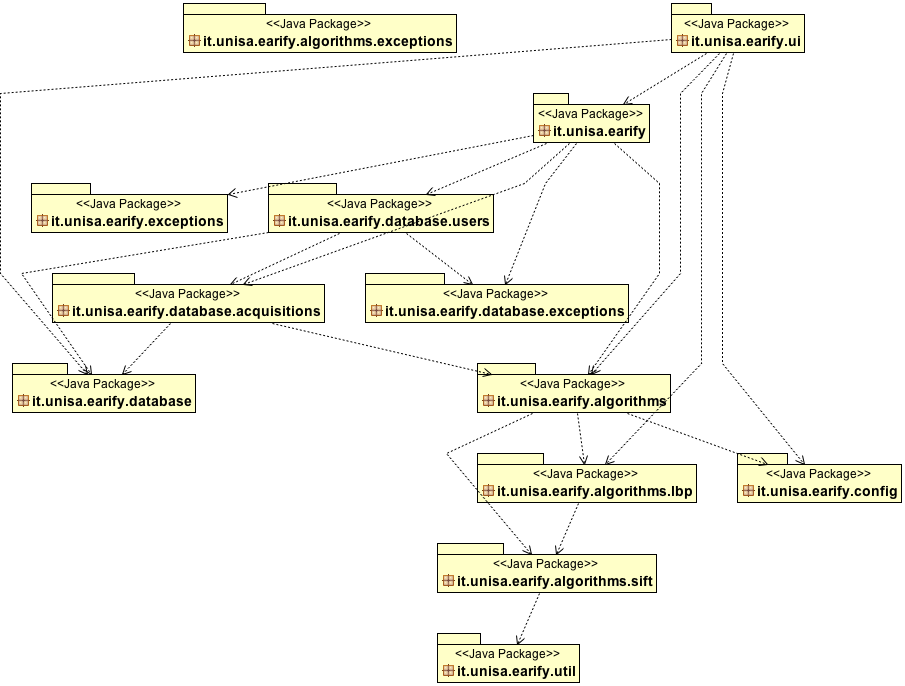
\includegraphics[width=1.5\textwidth, angle=90]{img/pkg.png}
	\caption{Packages}\label{fig:pkg}
\end{figure}

\section{Database}
L'accesso al database embedded nell'applicazione Android avviene tramite le classi diagrammate nella figura \ref{fig:db}.

\begin{figure}[ht]
	\centering
	%width=.5\textwidth
	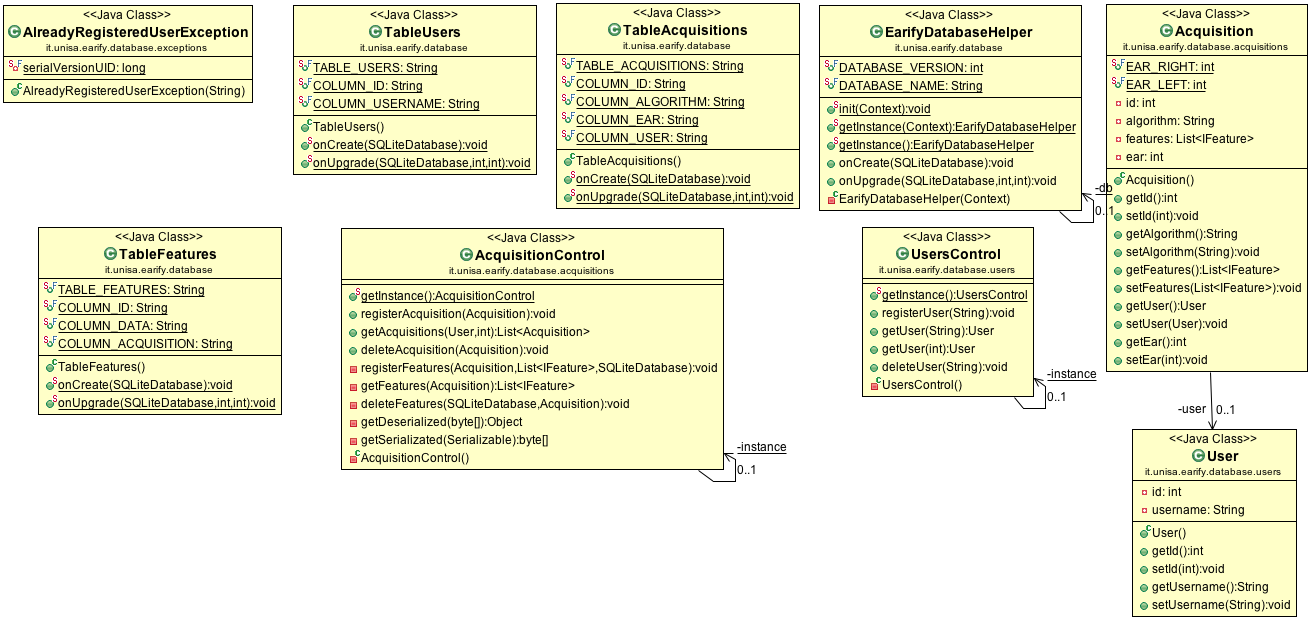
\includegraphics[width=1.5\textwidth, angle=90]{img/db.png}
	\caption{Classi database}\label{fig:db}
\end{figure}

